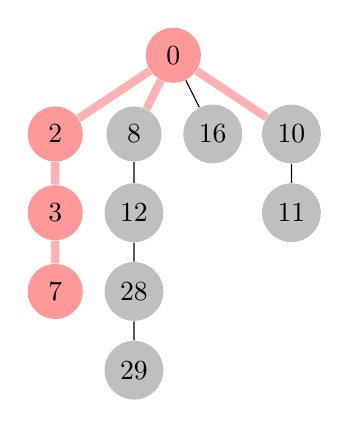
\begin{tikzpicture}[level/.style={sibling distance=10mm/#1, level distance=10mm}]
\tikzset{every node/.style={shape=circle,fill=black!25,minimum size=7mm}}
%\tikzset{every node/.style={shape=circle,
%                            font=\bfseries \Large,
%                            minimum size=3cm,
%                            scale=0.4
%                           }}
\node[fill=red!40] (root) {$0$}
    child {
        node[fill=red!40] {$2$}
        child {
            node[fill=red!40] {$3$}
            child {
                node[fill=red!40] {$7$
                };
                \path edge from parent[draw,line width=3pt,-,red!30];
            };
        \path edge from parent[draw,line width=3pt,-,red!30];
        };
    \path edge from parent[draw,line width=3pt,-,red!30];
    }
    child {
        node {$8$}
        child {
            node {$12$}
            child {
                node {$28$}
                child {node {$29$}
                }
            }
        };
    \path edge from parent[draw,line width=3pt,-,red!30];
    }
    child {node {$16$}}
    child {
        node {$10$}
        child {
            node {$11$}
        };
    \path edge from parent[draw,line width=3pt,-,red!30];
    }
    ;
\end{tikzpicture}
